% !TEX TS-program = pdflatex   
\documentclass[runningheads,12pt]{article} 
\usepackage{graphicx}
\usepackage{color,url}
\usepackage{mdframed}%put frame around text or a table
\usepackage{framed}
\usepackage{pdfpages}% Import pdf
\usepackage{soul}% Highlight
\usepackage{fancyvrb}

\usepackage[pdftex]{hyperref}
\usepackage{xurl}

\usepackage{sty/bsymb} %% Event-B symbols
\usepackage{sty/eventB} %% REQ and ENV
\usepackage{sty/b2latex}% Importing from Rodin
\usepackage{sty/calculation} % Calculational proofs
\newcommand{\term}[1]{\textit{#1}}

\usepackage{amsmath}
\usepackage{amsthm}
%\usepackage{mathtools}

\usepackage{fancyhdr,lastpage}
\lhead{\rm Greatest Common Divider in Eiffel}
\rhead {\rm Page \thepage~of \pageref{LastPage}}
\lfoot{}\cfoot{}\rfoot{}
\pagestyle{fancy}

% Listings needs package courier
\usepackage{listings} % Needs 
\usepackage{courier}
% Inline Eiffel Code
\newcommand{\e}[1]{\lstinline[language=eiffel]|#1|}

%Symbols
\def\Fl{\mathbb{F}}
\def\Rl{\mathbb{R}}
\def\Nl{\mathbb{N}}
\def\Bl{\mathbb{B}}
\def\St{\mathbb{S}}
\def\WD{\textrm{WD}}
\def\assert#1{\textcolor{red}{ {\{} {#1} {\}}}}

\usepackage{stmaryrd}
\def\b{\llbracket \rrbracket}
\def\a{\rightarrow}


\begin{document}

\title{Specifications and Implementation in Eiffel}
\author{Jonathan S. Ostroff \thanks{EECS, Lassonde School of Engineering, York University.}}
\date{\today}

\maketitle
\tableofcontents
\newpage

\section{Significance of Specifications and Formal Methods}
%%%%%%%%%%%%%%%%%%%%%%%%%%%%%%%%%%%%%%%%%%
It is non-trivial to develop reliable software products for safety-critical systems such as medical devices or nuclear power generation, concurrent systems or cybersecurity. For example:

\begin{quote}
Cybersecurity is everyone’s problem. The target may be the electric grid, government systems storing sensitive personnel data, intellectual property in the defense industrial base, or banks and the financial system. Adversaries range from small-time criminals to nation states and other determined opponents who will explore an ingenious range of attack strategies. And the damage may be tallied in dollars, in strategic advantage, or in human lives. Systematic, secure system design is urgently needed, and we believe that rigorous formal methods are essential for substantial improvements.

Formal methods enable reasoning from logical or mathematical \textit{specifications} of the behaviors of computing devices or processes; they offer rigorous proofs that all system behaviors meet some desirable property. They are crucial for security goals, because they can show that no attack strategy in a class of strategies will cause a system to misbehave. Without requiring piecemeal enumeration, they rule out a range of attacks. They offer other benefits too: Formal specifications tell an implementer unambiguously what to produce, and they tell the subsequent user or integrator of a component what to rely on it to do. Since many vulnerabilities arise from misunderstandings and mismatches as components are integrated, the payoff from rigorous interface specifications is large.\footnote{%
\textit{Report on the NSF Workshop on Formal Methods for Security}, 2016, \url{https://arxiv.org/pdf/1608.00678.pdf}. Italics not in the original.}
\end{quote}


\section{Example: Specifying and verifying Euclid's algorithm}
%%%%%%%%%%%%%%%%%%%%%%%%%%%%%%%%%%%%%%%%%%%%%%%%%%%%%

To understand the use of specifications and formal methods, we examine a simple example.  In mathematics, the Euclidean algorithm is an efficient method for computing the greatest common divisor (GCD) of two integers, the largest number that divides them both without a remainder. It is named after the ancient Greek mathematician Euclid, who first described it in his Elements (c. 300 BC). It is used in cryptographic computations to ensure the security of a variety of systems (\textit{Wikipedia}). 

\begin{figure}[!htb]
\begin{framed}
\begin{Verbatim}[fontsize=\small]
// golang
package main

import (
	"fmt"
)

// greatest common divisor (GCD) via Euclidean algorithm
// use only addition and subtraction 
func gcd(m, n int) int {
	x := m
	y := n
	for x != y {		// while loop
		if x < y {
			y = y - x
		} else {
			x = x - y
		}
	}
	return x
}

func main() {
	fmt.Println(gcd( 111, 259))
	fmt.Println(gcd(-111, 259))
}	
\end{Verbatim}
\end{framed}
The statement \textcolor{red}{\e{fmt.Println(gcd(-111, 259))}} is non-terminating. One might add an assert or defensive programming, neither of which is ideal. 
\caption{GCD implemented in Go}
\label{fig:gcd-c}
\noindent\rule{\textwidth}{0.5pt}
\end{figure}

In the sequel, we provide the text of an Eiffel program that contains \textit{specification} and  \textit{implementation} for Euclid's GCD algorithm. The implementation can be checked against the specification via runtime assertion checking.\footnote{%
See \url{https://github.com/yuselg/3311-W20-Public/tree/master/euclid/code/eiffel}.} The use of Hoare logic (via preconditions and postconditions) was invented at the dawn of software engineering. Design by Contract (DbC) as implemented in languages such as Eiffel and Ada have taken this conceptual machinery and made it applicable to large industrial strength software systems. 
 
%%%%%%%%%%%%%

\subsection{Testing can show the presence of bugs, but not their absence}

In Fig.~\ref{fig:gcd-c}, Euclid's algorithm is implemented in Golang.\footnote{%
Try it at \url{https://play.golang.org}.}

There is a ``while" loop in the code of Fig.~\ref{fig:gcd-c}. How sure are we that this implementation always terminates? If it does terminate, how do we know it always terminates with the correct result?

\begin{figure*}[hbt]
  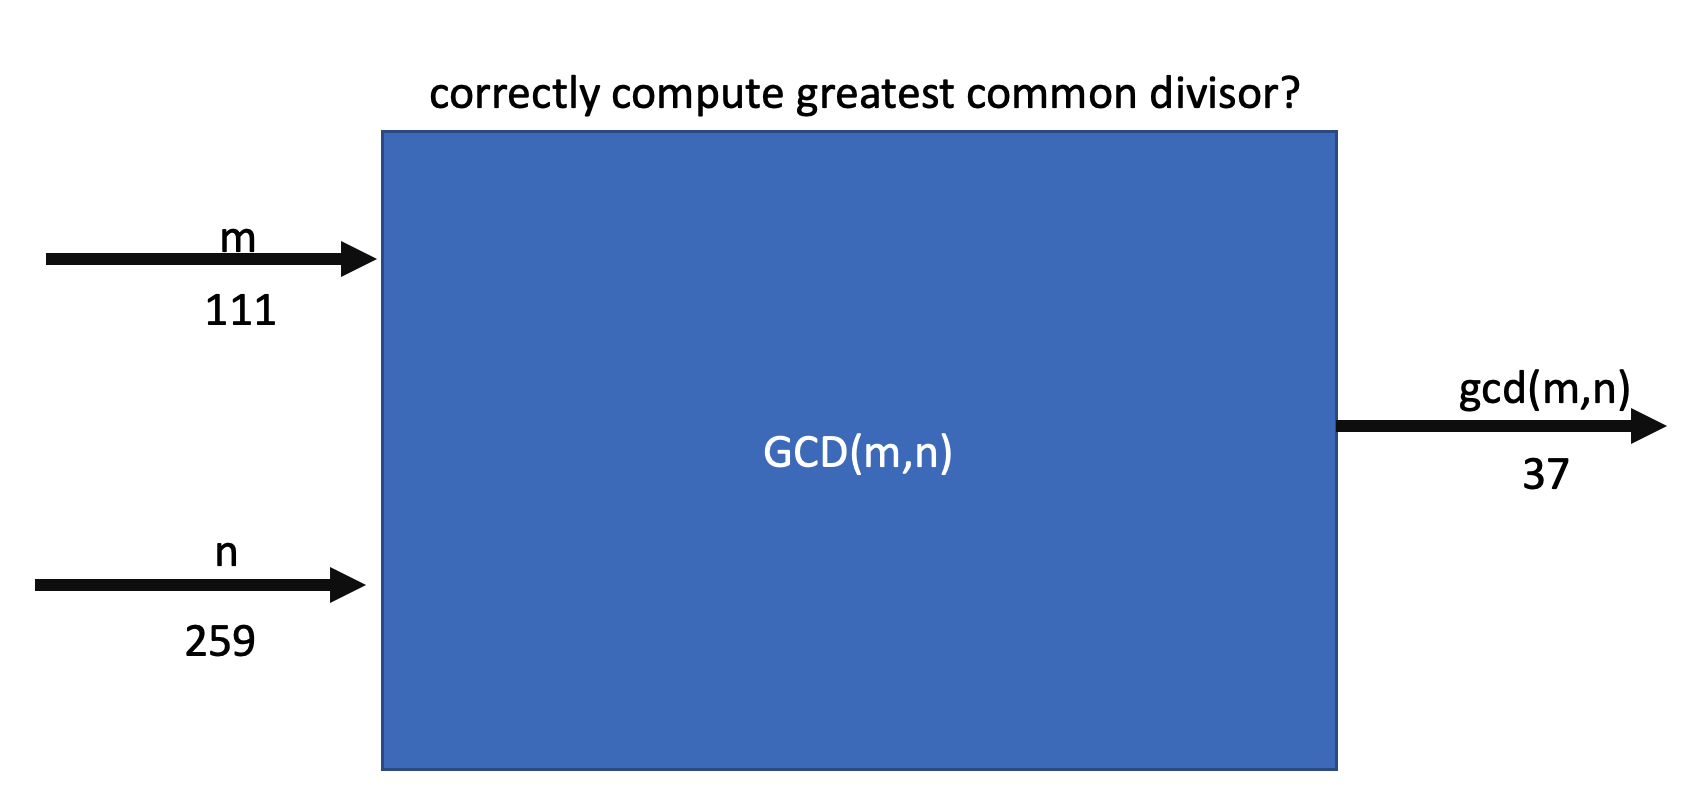
\includegraphics[width=0.8\textwidth]{images/gcd.png}
\end{figure*}


We can test the $gcd(m,n)$ subroutine. For example, we can provide inputs $m := 111$ and $n := 259$, and then we can check if the output is $gcd(111,259) = 37$. 

If we discover an an error in the code, then we can fix it. But here is the concern with testing alone: \textit{Dijkstra}: ``testing can show the presence of bugs, but not their absence". 

\begin{itemize}
  \item It does not matter how many tests we run, we can never exhaustively check the correctness of the algorithm. There are just too many combinations of inputs!
  \item To write a test, we also need to (manually?) compute the answer, a time consuming process. For example, to test gcd(111,259), we had to first manually compute the GCD by hand.\footnote{GCD is built-in in most programming languages. But we are assuming that, for the sake of illustration, that we are computing a new function, one for which there is no oracle.}
\end{itemize}

The earlier report (NSF Workshop on Formal Methods for Security) perhaps words it too strongly, but there is more than a grain of truth to it. Here is further quote from that report:

\begin{quote}
Formal methods are the only reliable way to achieve security and privacy in computer systems. Formal methods, by modeling computer systems and adversaries, can prove that a system is immune to entire classes of attacks (provided the assumptions of the models are satisfied). By ruling out entire classes of potential attacks, formal methods offer an alternative to the “cat and mouse” game between adversaries and defenders of computer systems.

Formal methods can have this effect because they apply a scientific method. They provide scientific foundations in the form of precise adversary and system models, and derive cogent conclusions about the possible behaviors of the system as the adversary interacts with it. This is a central aspect of providing a science of security.
\end{quote}

For a formal proof Euclid's algorithm in TLA+, see \url{https://lamport.azurewebsites.net/pubs/euclid.pdf}.  Tools such as TLA+ has been used at Amazon, Microsoft and elsewhere. 

\section{Correctness is relative to a Specification}
%%%%%%%%%%%%%%%%%%%%%%%%%%%%%%%%%%%%%%%%%%%%

To judge whether code is correct, we need a \textbf{specification}---this is something different from the Go \textbf{implementation} in Fig.~\ref{fig:gcd-c}. A specification is the software engineering equivalent of blue-prints in other engineering disciplines.

In Eiffel, we can specify the GCD algorithm using Design by Contract (DbC), as shown in Fig.~\ref{fig:gcd-spec}.

\begin{figure}[!htb]
\begin{framed}
\lstset{language=eiffel}    
\begin{lstlisting} 
gcd(m, n: INTEGER): INTEGER
		-- return the greatest common divider of $m$ and $n$
	require
		$m \geq 1 \land n \geq 1$ -- at least should not be zero
	ensure 
			gcd_spec: Result = $max(divisors(m) \binter divisors(n))$
	end
\end{lstlisting}
\end{framed}

The \e{require} clause is a precondition: $gcd$ is a partial function that is not well-defined for all possible inputs. For example, what is $gcd(0,0)$? So the precondition documents the fact that a client using this function must check that the precondition is true before calling it. Without loss of generality, our precondition is $m \geq 1 \land n \geq 1$.

\smallskip
The \e{ensure} clause is a postcondition. It asserts that the function must terminate with this condition true. But how shall we write this postcondition? In general, for that we need to define what a GCD is using predicate logic and set theory (with the help of the Mathmodels library).  

\begin{itemize}
  \item $divisors(n)$ is the set of all divisors of the number $n$. 
  \item $max(S)$ is the maximum of the set of numbers $S$. 
  \item $gcd\_spec(m,n)$ is the GCD of the numbers $m$ and $n$.
\end{itemize}

Formally, using set theory and predicate logic, we write

\begin{itemize}
  \item $divisors(q) \;\defi\; \{d \in 1 \upto q \mid divides(d, q)\}$, where $divides(d, q)$ is true if $d$ divides $q$, i.e. $q \mod d = 0$. 
  \item $gcd\_spec(m,n) \;\defi\; max(divisors(m) \binter divisors(n))$.
\end{itemize}

These specifications can themselves be written in an Eiffel-like form, e.g. $max(S)$ is as follows:

\begin{framed}
\begin{lstlisting}[language=eiffel]
max(s: SET[INTEGER]): INTEGER
	require $s \neq \emptyset$
	ensure $(Result \in s) \land (\forall i \in s \mid Result \geq i)$
\end{lstlisting}
\end{framed}
\caption{Specification of the GCD query in Eiffel}
\label{fig:gcd-spec}
\end{figure}
%%%%%%%%%%%%%%%%%%%%%%%%%%%%%%%%%%%%%%%%%%%%%%%%%%%%%%%%%%%%%%%%%

If the GCD query is invoked by a client in a manner that violates the precondition (e.g. \e{gcd(-111,259)}) then this illegal call will automatically terminate with a precondition violation:

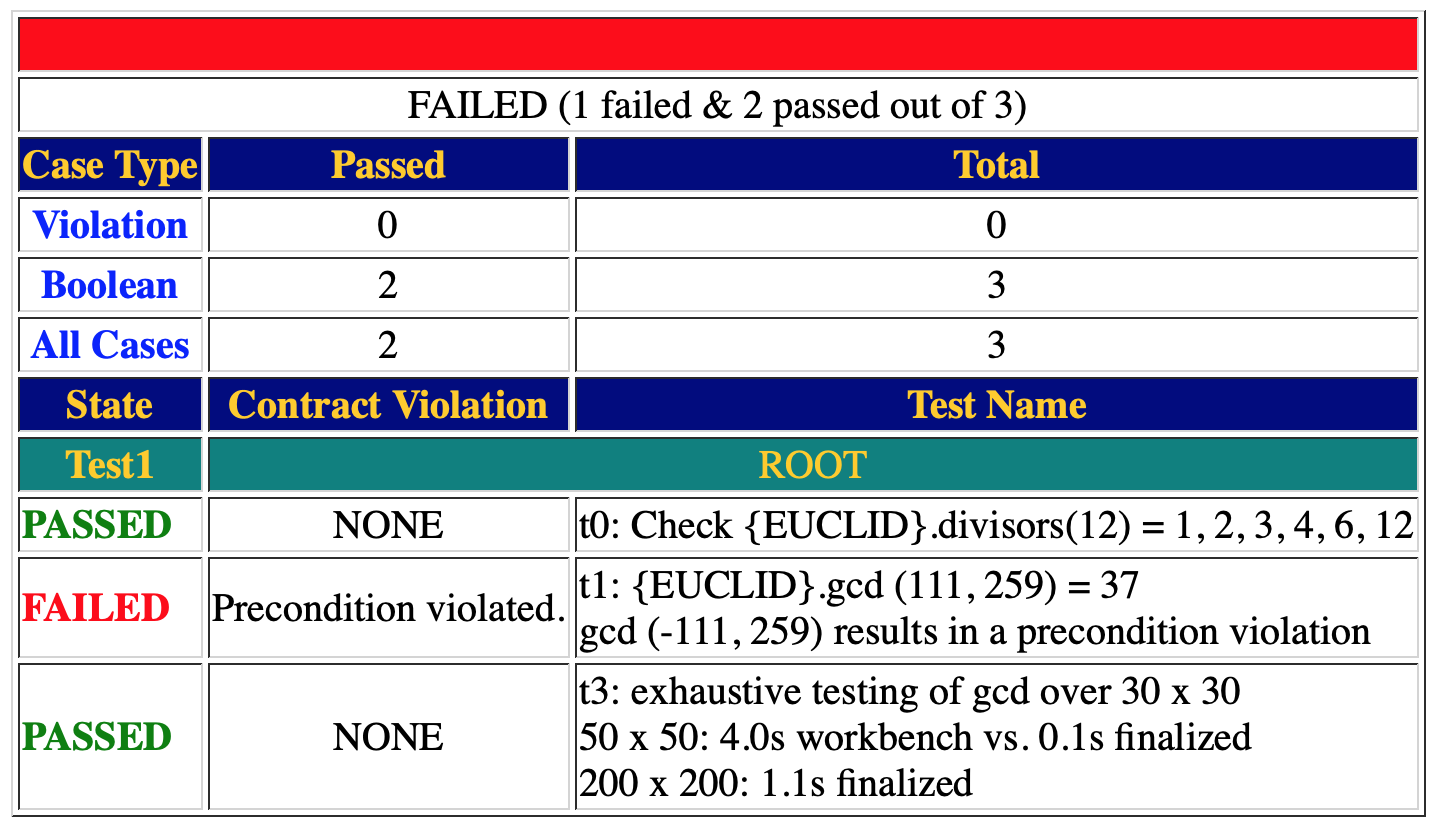
\includegraphics[width=.8\textwidth]{images/precondition-violate.png}

\subsection{Termination and Correctness} 

But we still need to prove that in the case the client makes a legal call, the GCD query terminates,  and terminates with the correct result (i.e. satisfies the specification).

To prove termination and correctness, we must provide the implementation with a loop \textbf{variant} (i.e. $x +y$) and \textbf{loop invariant} (i.e. $gcd\_spec(x,y) = gcd\_spec(m,n)$) as shown in Fig.~\ref{fig:gcd}.

%%%%%%%%%%%%%%%%%%%%%%%%%%%%%%%%%%%%%%%%%%%%%%%%%%%%%%%%%%%%%%%%%
\begin{figure}[!htb]
\begin{framed}
\caption{Specification and implementation of the GCD query in Eiffel}
\label{fig:gcd}
\lstset{language=eiffel}    
\begin{lstlisting} 
gcd(m, n: INTEGER): INTEGER
		-- return the greatest common divider of $m$ and $n$
	require
		$m \geq 1 \land n \geq 1$ -- at least should not be zero
	local
		x, y: INTEGER
	do
		from
			x := m; y := n
		invariant 
			inv: gcd_spec(x,y) = gcd_spec(m,n)
		until
			x = y
		loop
			if x < y then
				y := y - x
			else -- $\assert{y < x \;\textrm{as}\; x \neq y}$ 
				x := x - y
			end
		variant x + y
		end
		check x = y and x = gcd_spec(m,n) end
		Result := x
	ensure 
			Result = gcd_spec(m,n)
	end
\end{lstlisting} 
\end{framed}
\end{figure}

%%%%%%%%%%%%%%%%%%%%%%%%%%%%%%%%%%%%%%%

\section{Hoare Logic}
%%%%%%%%%%%%%%%%%%%%%%%%%%%%%%%%%%%%%%%%%%%%%

 We use the notation of a Hoare triple $\{Q\} S \{R\}$ where $Q$ is a precondition, $S$ is a program statement (i.e. code) and $R$ is a postcondition. 

\begin{quote}
[HT] Hoare Triple $\{Q\} S \{R\}$: Execution of the program statement $S$ begun in a state satisfying predicate $Q$ must (1) terminate, and (2) terminate in a state satisfying the predicate $R$. 	
\end{quote}

For example, let $S$ be the assignment statement ``$x := x - y$". Then we might write $\{x > 2y\}\; x := x - y \;\{x > y\}$. This Hoare Triple (HT) is \textit{valid}, i.e. execution of $x := x - y$ begun in a state satisfying $x > 2y$ is guaranteed to terminate in a state satisfying $x > y$.

The following HTA (Hoare Triple Assignment) Rule captures this type of logic:

\begin{gather}
\{R[x := exp] \land \WD(exp)\}\; x := exp \;\{R\} \tag{HTA}
\end{gather}

\noindent In the above, $R[x := exp]$ is a predicate similar to $R$, except that all free occurrences of variables $x$ in $R$ are replaced with expression $exp$.\footnote{Provided there is no illegal capture, see \cite{Tourlakis2008}. This can be extended to simultaneous replacement in the obvious manner: $R[x, y := exp1, exp2]$.} 

$\WD(exp)$ means that $exp$ must be well defined. For example, the expression $1/x$ is not well-defined if $x=0$; it is a partial function, not a total function. Thus $\WD(1/x) \1\equiv x \neq 0$.

In many cases, $\WD(exp) \1\equiv true$; thus, $R[x := exp] \land \WD(exp) \1\equiv  R[x := exp]$. We know from elsewhere that $R[x := exp] \land \WD(exp)$ is the weakest precondition such that executing $x := exp$ terminates with R true. For simplicity, we will use $R[x := exp]$ as the weakest precondition---and, we only mention $\WD(exp)$ in a context in which $exp$ is a partial function. The proof obligation HPA-PO to show that an assignment satisfies its specification is as follows:
\begin{quote}
[HTA-PO] To prove that the assignment $x := exp$ satisfies the Hoare specification $\{Q\}\; x := exp \;\{R\}$, it suffices to show that $Q \1\limp R[x :=exp]$. 
\end{quote}


\section{Proof of Termination and Correctness}\label{proofs}
%%%%%%%%%%%%%%%%%%%%%%%%%%%%%%%%%%%%%%%%%%%%%%%%%%%%%%%%%%%%

To understand a loop, and to prove that it terminates correctly, it is crucial to discover a loop invariant $inv$ (for partial correctness) and loop variant $t$ (an integer valued expression) for termination. We distinguish between partial correctness, which requires that if an answer is returned it will be correct, and total correctness, which additionally requires that the algorithm terminates.\footnote{Since there is no general solution to the halting problem, there is no guarantee that we can prove total correctness. However, loop variants and invariants have often been provided. See \cite{Gries1993,Gries1985} for deriving invariants for proof-by-construction.} 

This \textit{separates the concerns} of termination and correctness. There are five proof obligations; the first three prove partial correctness as shown in Fig.\ref{fig:gcd-loop-template}.

\begin{figure}[!htb]
\caption{Proof obligations for the termination and correctness of a loop}
\label{fig:gcd-loop-template}
\begin{tabular}{|p{0.3\textwidth}|p{0.65\textwidth}|}
\hline
\begin{lstlisting}[language=eiffel,numbers=left,firstnumber=0]
from
	$\assert{Q}$
	init
	$\assert{inv}$
until
	B  -- exit condition 
loop
	$\assert{inv \land \lnot B}$
	body
	$\assert{inv}$
variant $t$
end
$\assert{ inv \land B}$
$\assert{ R }$
\end{lstlisting}
 &  
 \footnotesize
\begin{enumerate}
  \item $\{Q\}\; \texttt{init} \;\{inv\}$: Given the precondition $Q$, show that the loop invariant is established initially (before execution of the loop begins).
  \item $\{inv \land \lnot B\}\; \texttt{body} \;\{inv\}$: Show that each execution of the loop body preserves the invariant. 
  \item $inv \land B \1\limp R$: On termination (i.e. $B$ holds), the invariant and the exit condition entail the postcondition $R$.
  \item $\{inv \land \lnot B \land t = T_0\}\; \texttt{body} \;\{t < T_0\}$ where $T_0$ is a constant: every execution of the loop results in a decrease of the variant $t$. 
  \item $inv \land \lnot B \1\limp t \geq 0$: Variant $t$ is bound from below, i.e. every execution of the loop may never cause the variant to become negative. 
\end{enumerate}
\\ \hline
\end{tabular}

\end{figure}





In Fig.~\ref{fig:gcd-loop}, we provide the fragment of the GCD code with the loop---annotated with Hoare assertion conditions (shown in \textcolor{red}{red}): 

\begin{figure}[!htb]
\begin{framed}
	\caption{Hoare annotations of the the GCD loop}
\label{fig:gcd-loop}
\begin{lstlisting}[language=eiffel,numbers=left,firstnumber=0]
from
	$\assert{precondition: m \geq 1 \land n \geq 1}$
	x, y := m, n  -- simultaneous assignment
	$\assert{ inv}$
invariant 
	inv: gcd_spec(x,y) = gcd_spec(m,n)
until
	x = y  -- exit condition B
loop
	if x < y then
		$\assert{ x < y \land inv}$ y := y - x $\assert{ inv}$
	else -- $\assert{y < x \;\textrm{as}\; x \neq y}$
		$\assert{ y < x \land inv}$ x := x - y $\assert{ inv}$
	end
variant t: x + y
end
$\assert{ x = y \land inv }$
$\assert{ x = gcd\_spec(m,n) }$
\end{lstlisting}
\end{framed}
\end{figure}


%There are five proof obligations that must be discharged to prove that the loop terminates, and terminates correctly. The first three proof obligations have to do with partial correctness, i.e. if we can assume termination, then:
%
%\begin{itemize}
%  \item the invariant \e{inv} is established initially;
%  \item each execution of the loop preserves the invariant;
%  \item thus, on termination the invariant and the exit condition entail line 17: $x = gcd\_spec(m,n)$.   
%\end{itemize}

The last two proof obligations show that the loop terminates. 
%%%%%%%%%%%%%%%%%%%%%%%%%%%%%%%%%%%%%%%%%%%%%

\subsection{Prove that the invariant $inv$ is established initially}

We must prove (see lines 1--3):


\begin{lstlisting}[language=eiffel]
    $\assert{ m \geq 1 \land n \geq 1}$
    x, y := m, n  -- simultaneous assignment
    $\assert{ inv}$
\end{lstlisting} 


\noindent By HTA-PO, it is sufficient to prove $m \geq 1 \land n \geq 1 \1\limp inv[x,y := m,n]$. We start with the consequent:
\vspace{-4pt}
\begin{calculation}
	inv[x,y := m,n]
\hint{\equiv}{definition of $inv: gcd\_spec(x,y) \1= gcd\_spec(m,n)$ and Leibniz}
	(gcd\_spec(x,y) = gcd\_spec(m,n))[x,y := m,n]
\hint{\equiv}{simultaneous assignment $gcd\_spec(x,y)[x,y := m,n] = gcd\_spec(m,n)$ and Leibniz}
	gcd\_spec(m,n) = gcd\_spec(m,n)
\hint{\equiv}{equality}
	true 
\hint{\Leftarrow}{propositional logic, strengthening}
	m \geq 1 \land n \geq 1 \qquad\blacksquare
\end{calculation}

	
%%%%%%%%%%%%%%%%%%%%%%%%%%%%%%%%%%%%%%%%
\subsection{Prove that each iteration of the loop preserves $inv$}

So long as we are in the loop, the negation of the exit condition holds, i.e. $x \neq y$. There are two branches to the conditional:

\begin{enumerate}
  \item $\assert{ x < y \land inv}$ y := y - x $\assert{ inv}$
  \item $\assert{ y < x \land inv}$ x := x - y $\assert{ inv}$
\end{enumerate}

\noindent We prove each branch separately. 

For the first branch, by HTA-PO, it is sufficient to prove $x < y \land inv \1\limp inv[y := y - x]$. We start with the consequent:
		
\begin{calculation}
	inv[y := y - x]
\hint{\equiv}{definition of $inv$ and Leibniz}
	(gcd\_spec(x,y) \1= gcd\_spec(m,n))[y := y - x]
\hint{\equiv}{assignment of free variables and Leibniz}
	gcd\_spec(x,y-x) \1= gcd\_spec(m,n)
\hint{\equiv}{GCD theorem: $y > x \1\limp gcd\_spec(x,y) = gcd\_spec(x,y-x)$}
	y > x \limp (gcd\_spec(x,y) \1= gcd\_spec(m,n))
\hint{\equiv}{definition of $inv$ and Leibniz}
	y > x \1\limp inv \qquad\blacksquare
\end{calculation}

The GCD theorem $y > x \2\limp gcd\_spec(x,y) = gcd\_spec(x,y-x)$ holds because any divisor of $x$ and $y$ is also a divisor of $x$ and $y-x$. We need $y > x$ to ensure that $\WD(gcd(x,y-x))$, so that $y-x \geq 1$.

The symmetric GCD theorem is $x > y \2\limp gcd\_spec(x,y) = gcd\_spec(x-y,y)$. Thus the second branch of the conditional can be proved symmetrically with the first. 

%%%%%%%%%%%%%%%%%%%%%%%%%%%%%%%%%%%%%%%

\subsection{Prove that exit condition and invariant entails postcondition} 

If the loop terminates (line 16), it must terminate with the exit condition true and the invariant must hold (as it has been shown to be preserved by every execution of the loop), i.e. we know: $x = y \1\land inv$.

We must now show that line 17 (i.e. $x = gcd\_spec(m,n)$) holds. We must thus show that $x = y \land inv \2\limp x = gcd\_spec(m,n)$.
	
\begin{calculation}
	x = y \1\land inv
\hint{\equiv}{definition of $inv$ and Leibniz}
	x = y \1\land gcd\_spec(x,y) = gcd\_spec(m,n)
\hint{\limp}{$x=y$ and Leibniz}	
	gcd\_spec(x,x) = gcd\_spec(m,n)
\hint{\equiv}{GCD Theorem: $gcd(x,x) = x$, obvious}
	x = gcd\_spec(m,n) \qquad\blacksquare
\end{calculation}

Finally, by HTA-PO, the following trivially holds:
\begin{lstlisting}[language=eiffel]
    $\assert{x = gcd\_spec(m,n)}$
    Result := x
    $\assert{Result = gcd\_spec(m,n)}$
\end{lstlisting} 

\noindent We have thus established the postcondition of $gcd(m,n)$.  

We have used various theorems about GCD in our proofs. We can prove these theorems using our GCD specification $gcd\_spec(x,y)$. To take a simple example, 

%TODO gcd(x,x)
\begin{calculation}
	gcd(x,x)
\hint{=} {definition $gcd\_spec(x,y)$}
	max(divisors(x) \binter divisors(x))
\hint{=}{set theory $A \binter A = A$}
	max(divisors(x))
\hint{=}{definition of divisors}
	max(\{d \in 1 \upto x \mid divides(d, x)\}
\hint{=}{definition of $max$}
	x
\end{calculation}

Thus, $(\forall x \geq 1: gcd(x,x) = x)$. $\qquad\blacksquare$

%%%%%%%%%%%%%%%%%%%%%%%%%%%%%%%%%%%%%%%

%%%%%%%%%%%%%%%%%%%%%%%%%%%%%%%%%%%%%%%%%
\subsection{Show that the variant decreases in each iteration}

Must show that: $\{inv \land \lnot B \land t = T_0\}\; loop \;\{t < T_0\}$, where $B$ is the exit condition of the loop. In the above, $T_0$ is an undetermined constant that represents the value of the variant at the beginning of each iteration. Left as an exercise.

\subsection{Show that the variant $t$ is bounded from below}

The variant $t$ is the integer expression $x+y$. So long as we are in the loop, $\lnot B$ holds where $B$ is the exit condition of the loop. We must thus show that $inv \land \lnot B \1\limp t \geq 0$. The truth is that we do not need the antecedent. We know that the precondition is $x \geq 1 \land y \geq 1$, so we can also trivially prove that $inv2: x \geq 1 \land y \geq 1$ is also a loop invariant. 

\begin{calculation}
	inv2: x \geq 1 \land y \geq 1
\hint{\limp} {arithmetic}
	x + y \geq 0
\hint{\equiv}{definition of $t$}
	t \geq 0 \qquad\blacksquare
\end{calculation}

\section{Eiffel: Exhaustive Runtime Assertion Checking}
%%%%%%%%%%%%%%%%%%%%%%%%%%%%%%%%%%%%%%%%
There is a ``lightweight" method of checking that the proofs hold for a bounded set of inputs, say $m \in 1\upto 100 \1\land n \in 1\upto 100$. This is similar to bounded but exhaustive modelchecking. 

The Eiffel runtime will automatically check all the assertions of Section~\ref{proofs}. In addition, any time we execute the query $gcd(m,n)$, all the contracts will be automatically checked, and violations will be reported.\footnote{%
The Eiffel program text with the specification and  implementation is provided at \url{https://github.com/yuselg/3311-W20-Public/tree/master/euclid/code/eiffel}}
This will provide us with confidence that the loop variant and invariant are well-posed and that the formal verification is feasible. Even without further formal verification, this may provide sufficient confidence in the software product beyond testing. 

\subsection{Specification Tests}
%%%%%%%%%%%%%%%%%%%%%%%%%%%%%%%

The specification $gcd\_spec(x,y)$ using Mathmodels is an executable specification (albeit inefficient) of the GCD. This specification can thus act as an Oracle in exhaustive testing as shown in Fig.~\ref{fig:spec-test} lines 12--15.

\begin{figure}[!htb]
\begin{framed}
\caption{Exhaustive Specification Test with Oracle gcd\_spec (line 15)}
\label{fig:spec-test}    
\begin{lstlisting}[language=eiffel,numbers=left,firstnumber=1]
	t3: BOOLEAN
		local
			euclid: EUCLID
			gcd, gcd_spec: INTEGER
			k: INTEGER -- iterations
		do
			comment (t3: exhaustive testing of gcd over 30 x 30)
			k := 30 -- use finalized for larger sets
			create euclid
			across 1 |..| k is m loop
			across 1 |..| k is n loop
				gcd := euclid.gcd (m, n)
				gcd_spec := euclid.gcd_spec (m, n)
				-- specification tests
 				Result := gcd = gcd_spec
 				check Result end
 			end
 			end
		end
\end{lstlisting}
\end{framed}
\end{figure}

Thus, writing a specification provides a method for writing automated tests beyond that of unit-testing. These concepts can be transferred over to testing written in other languages as well (depending on their ``expressivity"). When the software is deployed contract checking can be turn off for efficiency.

\section{Why Design by Contract?}
%%%%%%%%%%%%%%%%%%%%%%%%%%%%%%%%%

\begin{itemize}
  \item In the program text itself, write \textit{specifications} (not only implementations). 
  \item Documents the contract between client and supplier. See the contract view of the program text in Fig.~\ref{fig:contract-view}. There is a contract between the client and supplier, each having obligations and benefits. Loosely coupled objects are guaranteed to interact correctly with each other as specified in the contract.
  \item Verify that the implementation satisfies the \textit{specification}.
  \item Exhaustively test software products using Specification Tests. 
  \item Executions are raised only when there are contract violations. Avoids code bloat by eliminating the need for constant defensive programming. 
  \item  Subcontracting: ensures the Liskov substitution principle so that inheritance is used correctly. 
  \end{itemize}

As stated by Bertrand Meyer, Design by Contract can be used throughout the design process.\footnote{%
See \cite{Meyer1997a} for his description of Dbc.} 

\begin{quote}
	
The Eiffel method treats the whole process of software development as a continuum; unifying the concepts behind activities such as requirements, specification, design, implementation, verification, maintenance and evolution; and working to resolve the remaining differences, rather than magnifying them.

Formal specification languages look remarkably like programming languages; to be usable for significant applications they must meet the same challenges: defining a coherent type system, supporting abstraction, providing good syntax (clear to human readers and parsable by tools), specifying the semantics, offering modular structures, allowing evolution while ensuring compatibility.

The same kinds of ideas, such as an object- oriented structure, help on both sides. Eiffel as a language is the notation that attempts to support this seamless, continuous process, providing tools to express both abstract specifications and detailed implementations.\footnote{\url{https://bertrandmeyer.com/2014/12/07/lampsort/}.}
\end{quote}


\section{The Academy and Industry}
%%%%%%%%%%%%%%%%%%%%%%%%%%%%%%%%%%

Security researchers recently disclosed 19 vulnerabilities in a small library designed in the 90s that has been widely used and integrated into countless of enterprise and consumer-grade products over the last 20 years. 

The number of impacted products is estimated at ``hundreds of millions" and includes products such as smart home devices, power grid equipment, healthcare systems, industrial gear, transportation systems, printers, routers, mobile/satellite communications equipment, data center devices, commercial aircraft devices, various enterprise solutions, and many others.\footnote{%
\url{https://www.zdnet.com/article/ripple20-vulnerabilities-will-haunt-the-iot-landscape-for-years-to-come/}. Accessed 22 June 2020.}

From the description in the article, the three most serious vulnerabilities seem to be buffer overflows. C and C++ can be dangerous languages. For these devices, perhaps we should be using languages with strong static typing guarantees (e.g. Rust, Ada etc.). Even so, there is a way to use C safely if we have mastered disciplined programming methods discussed in this article. Such errors are easily avoidable but new vulnerabilities will continue to be built into products until programmers change the way they write and verify software. 

As pointed out by safety experts, ``thousands of development teams have incorporated these library routines in their products and, unsurprisingly, failed to find the vulnerabilities in their testing. Yet today, thousands of development teams will continue to resist using better methods, tools and languages".

Lesley Lamport writes that engineers draw detailed plans before a brick is laid or a nail is hammered. Programmers don’t. Can this be why houses seldom collapse and programs often crash?

Blueprints help engineers and architects to ensure that what they are planning to build will work. ``Working” means more than not collapsing; it means serving the required purpose. Engineers and their clients use blueprints to understand what they are going to build before they start building it. But few programmers write even a rough sketch of what their programs will do before they start coding.\footnote{%
\url{https://channel9.msdn.com/Events/Build/2014/3-642}. Lesley Lamport is the  author of TLA+ and winner of the Turing Award in 2013: \url{https://amturing.acm.org/award_winners/lamport_1205376.cfm}.
}

\subsection{Foundational Principles in CS/software engineering education}
\begin{quote}
Our recommendations are threefold, ... First, computer science majors, many of whom will be the designers and implementers of next-generation systems, should get a grounding in logic, ... “To designers of complex systems, the need for formal specs should be as obvious as the need for blueprints of a skyscraper. (Lesley Lamport) 

The methods, tools, and materials for educating students about ``formal specs" are ready for prime time. Mechanisms such as ``design by contract," now available in mainstream programming languages, should be taught as part of introductory programming, as is done in the introductory programming language sequence at Carnegie Mellon University. $\cdots$ We are failing our computer science majors if we do not teach them about the value of formal specifications.\footnote{%
``Teach Foundational Language Principles", Thomas Ball and Benjamin Zorn, \textit{Communications of the ACM}, May 2015, Vol. 58 No. 5, Pages 30-31. \url{https://cacm.acm.org/magazines/2015/5/186023-teach-foundational-language-principles/fulltext}. 

Thomas Ball (tball@microsoft.com) is a principal researcher and co-manager of the Research in Software Engineering (RiSE) group at Microsoft Research, Redmond, WA. Benjamin Zorn (zorn@microsoft.com) is a principal researcher and co-manager of the Research in Software Engineering (RiSE) group at Microsoft Research, Redmond, WA.} 
\end{quote}


%%%%%%%%%%%%%%%%%%%%%%%%%%%%%%%%%%%%%%%%
\bibliographystyle{alpha}
\bibliography{ref}
%%%%%%%%%%%%%%%%%%%%%%%%%%%%%%%%%%%%%%%%

\appendix

\section{Contract View of class EUCLID for GCD}

\begin{figure}[!htb]
\begin{framed}
\caption{Contract View of class EUCLID}
\label{fig:contract-view}
\lstset{language=eiffel}    
\begin{lstlisting}
class EUCLID feature

	gcd (m, n: INTEGER): INTEGER
			-- return the gcd of `m` and `n`
		require
			non_zero: m >= 1 and n >= 1
		ensure -- $Result = max(divisors(m) \binter divisors(n))$
			gcd_spec: Result = max(divisors(m) |/\| divisors(n))
	
feature -- gcd-spec

	divisors (n: INTEGER): SET [INTEGER]
			-- return set of divisors of `q`
		require
				n >= 1
		ensure -- $Result = \{d \in 1\upto q \mid is\_divisible (q, d)\}$
			divisors_set: Result $\sim$ (range (1, n) | agent is_divisible (n, ?))

	gcd_spec (m, n: INTEGER): INTEGER
			-- specification definition of gcd
		ensure
				Result = max (divisors (m) |/\| divisors (n))

	max (s: SET [INTEGER]): INTEGER
		require
				not s.is_empty
		ensure -- $(Result \in s) \1\land (\forall i \in s \mid Result \geq i)$
				contains: s.has (Result)
				is_max: across s is i all Result >= i end
end
				
\end{lstlisting}
\end{framed}
\end{figure}


\end{document}
